In diesem Teil werden alle theoretischen Informationen gegeben, die man für das Verständniss des ganzen Projektes braucht. Nach dieser Einführung sollte man in der Lage sein, den Quellcode im Anhang zu verstehen. Da es jedoch sehr viel Übung erfordert, einen Quellcode zu lesen und zu verstehen, ist es naheliegend, dass der Quellcode nicht verstanden wird. In der Einführung wird grob angeschaut, wie man überhaupt vom Quellcode zur App kommt, im zweiten Teil wird erklährt, wie Daten jeglicher Art als Zahlen in einem Computer abgespeichert werden, im dritten Teil gibt es eine Einführung in die Programmiersprache Java und im letzten Teil werden dann noch ein paar spezifische Informationen in bezug auf Java gegeben, die für die Erstellung einer App gebraucht werden und die Software "`Android Studio"' wird erklährt.

\subsection{Einführung}
\subsubsection{Die IDE}
Die IDE (eng. integrated development environment) oder auf Deutsch die Entwicklungsumgebung ist der Ort, an dem die meisten Programmierer arbeiten. Sie bietet alle wichtigen Werkzeuge, die man zum entwickeln von Software benötigt (Editor mit Color Highlighting, Compiler, Debugger, Dateibrowser etc.). Auf einige Begriffe wird später noch genauer eingegangen. In unserem Falle heisst die Entwicklungsumgebung übrigens Android Studio. In der Entwicklungsumgebung findet die ganze Entwicklung einer Software statt. Der wichtigste Bereich davon ist der Editor. Dort wird der ganze Quellcode hingeschriben und dank Color Highlighting werden die wichtigen Komponenten (Kontrollstrukturen, Variablen, Kommentare etc. siehe Abschnitt 2.3 Grundlagen von Java) mit Farbe hervorgehoben (Abbildung \ref{fig:Colorhighlighting}).
\begin{figure}[htbp] 
  \centering
     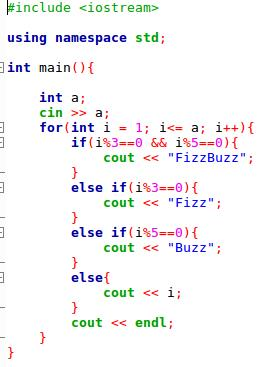
\includegraphics[width=0.3\textwidth]{CodeColor.jpg}
     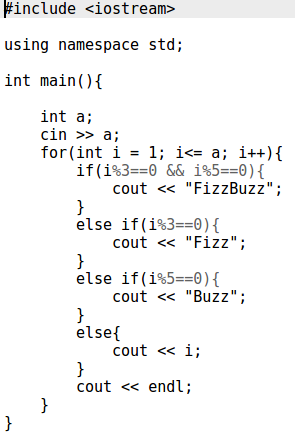
\includegraphics[width=0.3\textwidth]{CodeWithoutColor.png}
  \caption{Beispiel mit und ohne Farbhervorhebung \cite{Colorhighlighting}}
  \label{fig:Colorhighlighting}
\end{figure}
Das ist sehr wichtig, da man ansonsten schnell den Überblick verloren hat. Natürlich gibt es nicht nur eine IDE sondern ganz viele. Welche man davon benutzt ist jedem selbst überlassen. Es gibt auch Entwickler, die es bevorzugen, ohne eine IDE zu arbeiten. Zwar kann man dann alles selbst so gestallten wie es einem passt, es macht aber alles viel komplizierter ist besonders für neu beginnende Programmierer nicht empfehlenswert.

\subsubsection{Der Compiler}
Leider versteht der Computer nichts von dem, was wir in den Quellcode schreiben, alles was er versteht besteht aus Nullen und Einsen (mehr darüber im Abschnitt 2.2). Deshalb muss der für uns verständliche Quellcode in Maschinencode übersetzt werden. Dies geschieht mit dem so gennanten "`Compiler"' (eng. to compile = zusammentragen). Meistens ist dieser bereits in der IDE enthalten und auf Knopfdruck abrufbar. 

\subsubsection{Der Debugger}
Der Debugger ist sehr eng mit dem Compiler verbunden. Meistens schafft man es nähmlich nicht, auf Anhieb einen Fehlerlosen Code zu schreiben. Es passiert extrem schnell, dass irgendwo ein "`;"' oder eine Kontrollstruktur falsch geschrieben wurde (mehr dazu im Abschnitt 2.3). Deshalb ist es sehr wichtig, dass man den Fehler findet. Wenn man jetzt aber Quellcode von 500 Zeilen geschrieben hat, wäre es doch sehr mühsam, wenn man nur wüsste, dass man einen Fehler hat. Genau dafür ist der Debugger. Ist aus dem englischen Wort "`Bug"' entstanden, was so viel wie Käfer heisst, im Programmieren aber als Synonym zu Fehler verwendet wird. Dementprechend könnte man also Debugger als "`Entfehlerer"' oder verdeutscht als "`Fehlersuchprogramm"' bezeichnen. Meistens wird er aber einfach Debugger gennant. Offenbar ist der Debugger dazu in der Lage, die Programmierfehler zu finden. Er findet aber leider nur Syntaxfehler und keine, die den gewünschten Programmoutput betreffen. Man kann sich das so vorstellen: In Microsoft Word werden auch Rechtschreibefehler angezeigt, trotzdem kann man Sätze bilden die entweder keinen Sinn ergeben oder etwas anderes Aussagen, als gewünscht. Aber der Programmieraltag ohne Debugger wäre fast unvorstellbar, da man die meisten Fehler nicht so einfach sieht wie ein falsch geschriebenes Wort. Es gibt verschiedene Arten von Debugger. Die meisten zeigen einem die Fehler erst an, wenn man den Quellcode zu komplieren versucht, es gibt aber auch solche, die das in Echtzeit machen, so wie Microsoft Word Rechtschreibefehler anzeigt. 

\subsubsection{Die Programmiersprache}
Eine Programmiersprache kann man sich am einfachsten wie eine richtige Sprache vorstellen. Sie bildet den Grundbaustein des Programmierens. Bevor man dem Computer etwas  beibringen kann, muss man eine solche lernen. Jede Programmiersprache hat seine eigene Syntax, trotzdem sind sie meistens ähnlich aufgebaut. Sobald man also eine Programmiersprache gelernt hat, fällt es einem einfach, eine nächste zu lernen. Man muss sich das so vorstellen: Nachdem man gelernt hat, wie Windows XP funktioniert, hat man nicht mehr so grosse Schwierigkeiten, zu lernen wie Windows 7 oder Windows 8 funktioniert. Meistens haben die Programmiersprachen verschiedene Anwendungsbereiche: Wird z. B. JavaScript und PHP meist nur in Webanwendungen verwendet, wird C++ wegen seiner Geschwindigkeit meist in Systemanwendungen gebraucht oder Java für Geräte wie Drucker oder eben Androidapplikationen, ausserdem ist das berühmte Computerspiel "`Minecraft"' in Java geschrieben.
\subsection{Von der Zahl zum Bild}

\subsection{Grundlagen von Java}

\subsection{Android Studio}